\section{The design, derived from scratch}

Most write-ups \emph{show} you the final data structures. This one \emph{derives}
them --- starting from the dumbest thing that works and letting each operation's
pain force the next structure into existence. If you can reproduce this reasoning
on a whiteboard, you can defend every line of the code. We go one step at a time,
and nothing is assumed.

\subsection{Step 0 --- the dumbest thing that works}

Store every order in one list. That's it.

\begin{center}
\begin{tikzpicture}[font=\small]
  \node[draw,rounded corners,fill=Soft,align=left,inner sep=7pt] {%
    \ttfamily std::vector<Order> orders;\\[3pt]
    [\,\{O1,Sec1,Buy,1000,U1,A\},\ \{O2,Sec1,Sell,500,U2,A\},\ \dots\,]};
\end{tikzpicture}
\end{center}

Does it \emph{work}? Yes --- every operation is possible. Is it \emph{good}? No.
Let's stress each of the six operations against it and watch it break.

\begin{center}
\renewcommand{\arraystretch}{1.3}\footnotesize
\begin{tabular}{@{}lll@{}}
\toprule
\textbf{Operation} & \textbf{On a plain vector} & \textbf{Cost} \\
\midrule
\code{addOrder} & \code{push\_back} & O(1) --- fine \\
\code{cancelOrder(id)} & scan the whole vector to find the id & \textcolor{Sell}{O(n)} \\
\code{cancelOrdersForUser} & scan, test each \code{user} & \textcolor{Sell}{O(n)} \\
\code{cancelOrdersForSecId\dots} & scan, test each \code{securityId} & \textcolor{Sell}{O(n)} \\
\code{getMatchingSizeForSecurity} & scan + do the matching maths & \textcolor{Sell}{O(n)} \\
\code{getAllOrders} & copy the vector & O(n) --- unavoidable \\
\bottomrule
\end{tabular}
\end{center}

\begin{intu}
Five of the six operations are $O(n)$ scans. With a million orders and repeated
queries, that is death by a thousand linear passes. Every improvement below is
just: \emph{``stop scanning --- keep an index that already knows the answer.''}
\end{intu}

\subsection{Step 1 --- fix \texttt{cancelOrder}: index by id}

\code{cancelOrder} is handed only an \emph{id}. To avoid scanning, we need to jump
from id straight to the order. That's the definition of a hash map:

\begin{center}
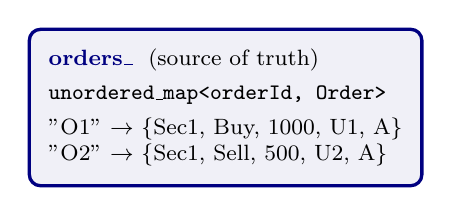
\begin{tikzpicture}[font=\footnotesize]
  \node[draw=NavyBlue,very thick,rounded corners,fill=NavyBlue!6,align=left,inner sep=7pt]{%
    \textbf{\color{NavyBlue}orders\_}\ \ (source of truth)\\[3pt]
    \ttfamily unordered\_map<orderId, Order>\\[3pt]
    "O1" \(\to\) \{Sec1, Buy, 1000, U1, A\}\\
    "O2" \(\to\) \{Sec1, Sell, 500, U2, A\}};
\end{tikzpicture}
\end{center}

Now \code{cancelOrder} is \code{orders\_.erase(id)} --- O(1) average. This map is
also our \textbf{single source of truth}: from here on, every other structure is
\emph{derived} from it and must be kept consistent with it.

\subsection*{Aside --- why is a hash map ``O(1)''? (for the layman)}
\addcontentsline{toc}{subsection}{\quad Aside: why a hash map is O(1)}

A \code{std::unordered\_map} is an array of \emph{buckets}. To store key\,$\to$\,value
it runs the key through a \emph{hash function} --- a scrambler that turns
``\code{O2}'' into a number --- then takes that number modulo the array size to
pick a bucket, and drops the entry there.

\begin{center}
\begin{tikzpicture}[font=\footnotesize,>=Latex,node distance=3mm]
  \node (k) {\ttfamily "O2"};
  \node[draw,rounded corners,fill=Accent!12,right=6mm of k] (h) {hash()};
  \node[right=6mm of h] (n) {\ttfamily 91823};
  \node[draw,rounded corners,fill=Gold!12,right=6mm of n] (m) {\% 8};
  \node[right=5mm of m] (b) {bucket \ttfamily 7};
  \draw[->](k)--(h);\draw[->](h)--(n);\draw[->](n)--(m);\draw[->](m)--(b);
  \node[draw,rounded corners,fill=Soft,right=6mm of b,align=left,inner sep=4pt]
    {\ttfamily [0][1]\dots[7]$\to$\{O2\}\dots};
\end{tikzpicture}
\end{center}

\begin{itemize}[leftmargin=1.4em,nosep]
  \item \textbf{Lookup/insert/erase} = hash the key, jump to that one bucket, done.
        No scan of the other entries --- that's the \textbf{O(1)} part.
  \item \textbf{Collisions} (two keys landing in the same bucket) are handled by a
        short list in that bucket. As long as the table keeps the average bucket
        tiny --- it resizes when the \emph{load factor}, entries$\div$buckets, gets
        high --- those lists stay length $\approx1$.
  \item That's why it's ``\textbf{O(1) \emph{average}},'' not guaranteed: a bad hash
        or a rare all-collide case degrades to O(n). For our string ids with the
        standard hash, average O(1) is the honest expectation.
\end{itemize}

\begin{intu}
Contrast with \code{std::map} (a balanced tree): it keeps keys \emph{sorted}, so
lookup is O($\log n$). We never need sorted order here, so we pay nothing for it
and take the faster O(1) hash map. \emph{Choosing \code{unordered\_} over ordered
is itself a deliberate, defensible decision.}
\end{intu}

\begin{keybox}[The source-of-truth principle]
Exactly one structure \emph{owns} the order data (\code{orders\_}). Everything
else is a lookup shortcut that \emph{points into} it. If two structures both
claimed to own the data, they could disagree --- so we never let that happen.
\end{keybox}

\subsection{Step 2 --- fix the targeted cancels: index by user and by security}

\code{cancelOrdersForUser} is handed a \emph{user}; \code{cancelOrdersForSecId\dots}
a \emph{security}. Same disease, same cure: keep a map from that key to the set of
ids that have it, so we touch only the relevant orders instead of scanning all $n$.

\begin{center}
\begin{tikzpicture}[font=\footnotesize,>=Latex,node distance=8mm]
  \node[draw=Buy,thick,rounded corners,fill=Buy!6,align=left,inner sep=6pt] (usr)
    {\textbf{\color{Buy}ordersByUser\_}\\[2pt]
     \ttfamily map<user, set<orderId>>\\[2pt]
     "U1" \(\to\) \{O1\}\quad "U2" \(\to\) \{O2\}};
  \node[draw=Sell,thick,rounded corners,fill=Sell!6,align=left,inner sep=6pt,right=1.4cm of usr] (sec)
    {\textbf{\color{Sell}ordersBySecurity\_}\\[2pt]
     \ttfamily map<secId, set<orderId>>\\[2pt]
     "Sec1" \(\to\) \{O1, O2\}};
\end{tikzpicture}
\end{center}

Why a \code{set} of ids, not a \code{vector}? Because a cancel must \emph{remove}
one id, and removing from a hash set is O(1); from a vector it's O(k). And a set
naturally forbids duplicates.

\begin{intu}
These two maps are \textbf{secondary indexes}, exactly like an index in a
database: they don't hold the data, they hold \emph{pointers} (ids) to it, so a
``find all rows where user = U2'' is instant instead of a full-table scan.
\end{intu}

Now \code{cancelOrdersForUser("U2")} is: look up \code{\{O2\}}, delete just those.
O(k) where $k$ is that user's order count --- not O(n).

\subsection{Step 3 --- the hard one: make matching fast \emph{without} scanning}

\code{getMatchingSizeForSecurity} still scans. Can an index save us? Not directly
--- matching isn't a lookup, it's a \emph{computation} over all of a security's
orders. But recall the formula (\S3):
\[
M=\min\Big(\sum_c\min(\text{buy}_c,\ S-\text{sell}_c),\ \min(B,S)\Big).
\]
Look at what it actually needs: \emph{not} the individual orders, only a handful
of \textbf{sums} per security --- the total buy $B$, total sell $S$, and each
company's buy and sell. If we keep those sums \emph{continuously updated}, the
query never looks at an order at all.

\begin{center}
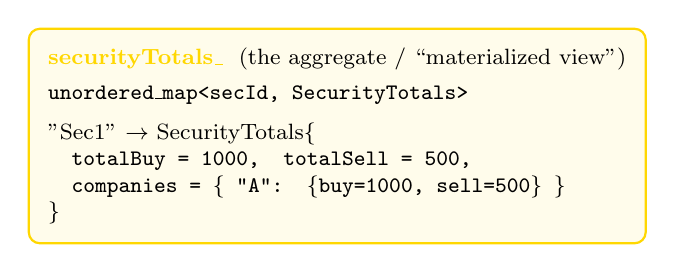
\begin{tikzpicture}[font=\footnotesize]
  \node[draw=Gold,thick,rounded corners,fill=Gold!8,align=left,inner sep=7pt]{%
    \textbf{\color{Gold}securityTotals\_}\ \ (the aggregate / ``materialized view'')\\[3pt]
    \ttfamily unordered\_map<secId, SecurityTotals>\\[5pt]
    "Sec1" \(\to\) SecurityTotals\{\\
    \quad\ttfamily totalBuy = 1000,\ \ totalSell = 500,\\
    \quad\ttfamily companies = \{\ "A": \{buy=1000, sell=500\}\ \}\\
    \}};
\end{tikzpicture}
\end{center}

The nested type is tiny and purpose-built --- it is \emph{exactly} the state the
formula consumes:

\begin{lstlisting}
struct CompanyTotals  { std::uint64_t buy = 0, sell = 0; };
struct SecurityTotals {
    std::uint64_t totalBuy = 0, totalSell = 0;
    std::unordered_map<std::string, CompanyTotals> companies;   // per-company buy/sell
};
\end{lstlisting}

\begin{keybox}[The key move: trade a little write-time work for O(1)-ish reads]
Instead of computing the sums \emph{at query time} (a scan), we maintain them
\emph{at write time}. Every \code{addOrder} adds its \code{qty} to two totals; every
cancel subtracts them. The query then just folds over the (few) companies --- it
is $O(\#\text{companies in that security})$, which is tiny and independent of $n$.
This is called a \textbf{materialized view}: a pre-computed answer kept fresh on
every write.
\end{keybox}

\subsection{Step 4 --- the assembled design (all four structures)}

\begin{center}
\begin{tikzpicture}[font=\footnotesize,>=Latex,node distance=6mm]
  \node[draw=NavyBlue,very thick,rounded corners,fill=NavyBlue!6,align=left,inner sep=6pt] (truth)
    {\textbf{\color{NavyBlue}orders\_}\ (source of truth)\\
     \ttfamily unordered\_map<orderId, Order>};
  \node[draw=Buy,thick,rounded corners,fill=Buy!6,align=left,inner sep=6pt,below left=1.1cm and -2.2cm of truth] (usr)
    {\textbf{\color{Buy}ordersByUser\_}\\\ttfamily <user, set<orderId>>};
  \node[draw=Sell,thick,rounded corners,fill=Sell!6,align=left,inner sep=6pt,below=1.1cm of truth] (sec)
    {\textbf{\color{Sell}ordersBySecurity\_}\\\ttfamily <secId, set<orderId>>};
  \node[draw=Gold,thick,rounded corners,fill=Gold!8,align=left,inner sep=6pt,below right=1.1cm and -2.2cm of truth] (agg)
    {\textbf{\color{Gold}securityTotals\_}\\\ttfamily <secId, SecurityTotals>};
  \draw[->,Buy] (usr) -- (truth); \draw[->,Sell] (sec) -- (truth); \draw[->,Gold] (agg) -- (truth);
  \node[below=1.4cm of sec,font=\itshape\color{gray},align=center]
    {the three derived structures all reference / summarize the one source of truth};
\end{tikzpicture}
\end{center}

\begin{center}
\renewcommand{\arraystretch}{1.3}\footnotesize
\begin{tabular}{@{}p{3.9cm}p{5.6cm}p{3.6cm}@{}}
\toprule
\textbf{Structure} & \textbf{Type} & \textbf{Makes fast} \\
\midrule
\code{orders\_} & \code{unordered\_map<orderId, Order>} & cancelOrder, getAllOrders \\
\code{ordersByUser\_} & \code{<user, unordered\_set<orderId>>} & cancelOrdersForUser \\
\code{ordersBySecurity\_} & \code{<secId, unordered\_set<orderId>>} & the per-security cancel \\
\code{securityTotals\_} & \code{<secId, SecurityTotals>} & getMatchingSizeForSecurity \\
\bottomrule
\end{tabular}
\end{center}

\subsection{Step 5 --- the catch, and the rule that tames it}

We now have \textbf{four} structures describing the same orders. The danger:
they can \emph{drift apart}. If \code{addOrder} inserts into \code{orders\_} and
\code{ordersBySecurity\_} but forgets \code{securityTotals\_}, matching silently
returns wrong numbers forever.

The rule that prevents this: \textbf{all mutation flows through exactly two private
helpers}, and nothing else ever touches an index or the aggregate.

\begin{center}
\begin{tikzpicture}[font=\footnotesize,>=Latex,node distance=5mm,every node/.style={align=center}]
  \node[draw,rounded corners,fill=Buy!8] (add) {addOrder};
  \node[draw,rounded corners,fill=Sell!8,below=6mm of add] (c1) {cancelOrder};
  \node[draw,rounded corners,fill=Sell!8,below=2mm of c1] (c2) {cancelForUser};
  \node[draw,rounded corners,fill=Sell!8,below=2mm of c2] (c3) {cancelForSec\dots};
  \node[draw=Accent,thick,rounded corners,fill=Accent!12,right=2.2cm of add] (ins) {\textbf{insertOrderInternal}\\updates all 4};
  \node[draw=Accent,thick,rounded corners,fill=Accent!12,right=2.2cm of c2] (rem) {\textbf{removeOrderInternal}\\updates all 4};
  \draw[->](add)--(ins);
  \draw[->](c1)--(rem);\draw[->](c2)--(rem);\draw[->](c3)--(rem);
\end{tikzpicture}
\end{center}

\begin{keybox}[Single point of truth for invariants]
Because every insert goes through \code{insertOrderInternal} and every removal
through \code{removeOrderInternal}, there is exactly \emph{one} place each can go
wrong --- and it's under your eye. The three cancel methods differ only in
\emph{which ids} they select; the actual deletion is the same shared code. Less
code to be wrong = fewer bugs.
\end{keybox}

\subsection{Step 6 --- final complexity scorecard}

\begin{center}
\renewcommand{\arraystretch}{1.3}
\begin{tabular}{@{}lll@{}}
\toprule
\textbf{Operation} & \textbf{Step 0 (vector)} & \textbf{Final design} \\
\midrule
addOrder & O(1) & O(1) avg (insert + 3 updates) \\
cancelOrder & \textcolor{Sell}{O(n)} & \textcolor{Buy}{O(1) avg} \\
cancelOrdersForUser & \textcolor{Sell}{O(n)} & \textcolor{Buy}{O(k)} \\
cancelOrdersForSecId\dots & \textcolor{Sell}{O(n)} & \textcolor{Buy}{O(k)} \\
getMatchingSizeForSecurity & \textcolor{Sell}{O(n)} & \textcolor{Buy}{O(\#companies)} \\
getAllOrders & O(n) & O(n) (unavoidable) \\
\bottomrule
\end{tabular}
\end{center}

\begin{intu}
We turned five $O(n)$ scans into $O(1)$/$O(k)$/$O(\#\text{companies})$ operations,
paying only a small constant of extra bookkeeping per write and $O(n)$ extra
memory for the indexes. With a million orders and frequent matching queries, that
is exactly the trade you want --- and being able to \emph{name} it (write-time cost
for read-time speed; a materialized view) is the senior signal.
\end{intu}

\begin{say}
``I start from a single source-of-truth hash map by id, add secondary indexes by
user and by security so the targeted cancels touch only relevant orders, and keep
a per-security aggregate --- totals plus per-company buy/sell --- as a materialized
view so matching is an $O(\#\text{companies})$ fold instead of a scan. All four
structures are kept in lockstep through two private helpers, so they can't drift.
It's a tiny hand-rolled database: one table, two indexes, one materialized view.''
\end{say}
